% This paper tries to present the thermodynamic point of view for studying the transportation system. To show the universe of this contribution, a general transportation model is used instead of the previous linear one.

% This new point of view is to analogize the transportation system to the thermodynamic system. The fundamental pair of correspondent concepts are the vehicle and the energy. The principles are introduced as well.

% The approach of Shannon's entropy is also explored to present the notion of transportation information, which measures the system contribution to the transportation functionality.

% preprint format
\documentclass[preprint,authoryear,12pt]{elsarticle}
% final format
% \documentclass[final,authoryear,5p,times,twocolumn]{elsarticle}
% \journal{}

% postScript packages and setting
\usepackage{graphicx}
\usepackage{ifpdf}
\ifpdf
\DeclareGraphicsExtensions{.pdf,.jpeg,.png}
\usepackage[bookmarks=true,colorlinks=true]{hyperref}
\else
\DeclareGraphicsExtensions{.eps}
\usepackage[bookmarks=true,colorlinks=true,dvipdfmx]{hyperref}
\fi
\usepackage{subfigure}

% mathematic packages and settings
\usepackage{amsmath}
\usepackage{amssymb}
\usepackage{amsthm}
\renewcommand{\vec}[1]{\mbox{\boldmath$#1$}}
\newcommand{\mat}[1]{\mbox{\boldmath$#1$}}
\newcommand{\unit}[1]{\,\mathrm{#1}}
\newtheorem{thm}{Theorem}
\newtheorem{lmm}{Lemma}
\newtheorem{ass}{Assumption}
\newtheorem{rmk}{Remark}
\newtheorem{dfn}{Definition}
\newtheorem{prpn}{Proposition}

\begin{document}

\begin{frontmatter}

\title{Thermodynamic and Information Theory Point of View for Urban
Transportation Network}
\author[SeT]{Huide Zhou\corref{cor}}
\ead{huide.zhou@utbm.fr}
\author[SeT]{Rachid Bouyekhf}
\ead{rachid.bouyekhf@utbm.fr}
\author[SeT]{Adbellah EL Moudni}
\ead{abdellah.el-moudni@utbm.fr}
\address[SeT]{Laboratoire Syst\`{e}mes et Transports (SeT),\\
Universit\'{e} de Technologie de Belfort-Montb\'{e}liard (UTBM)\\
Rue Thierry Mieg, 90010 Belfort Cedex, France}
\cortext[cor]{Corresponding author.}

\begin{abstract}
To explore the nature of the transportation system, this paper shows the connections between transportation systems and thermodynamic systems by regarding the vehicles as the energy supplied to the system. The correspondence of basic concepts are also presented, and it is demonstrated that transportation systems can have a similar notion of entropy to measure the system disorder. In addition, it is shown that, though the second law of thermodynamics can not be introduced directly into the transportation context, a similar dissipativity phenomenon of the transportation entropy  reduces the system disorder and hence renders the system  better organized.
% the principles of thermodynamics are also introduced into the transportation context. , the second law of thermodynamics leads to a dissipative law of the transportation entropy which can make the transportation system tend to reduce its disorder and hence become better organized.
Furthermore, the approach of Shannon's entropy is also applied in this paper to present the concept of the information in transportation context. It is shown that Shannon's entropy can measure the transportation functionality  and hence can be a good means to evaluate the system. 
% With all these efforts, this paper provides a novel thermodynamic and information point of view for the urban transportation network.
\end{abstract}

\begin{keyword}
Transportation systems\sep thermodynamic system \sep entropy\sep dissipativity theory\sep Shannon \sep information theory.
\end{keyword}

\end{frontmatter}

\section{Introduction}

Urban transportation is an essential part of the modern cities. Due to the rapid increase of traffic demands in recent decades, the congestion problem has become very frequent and led to serious economic and environment issues.

To solve it, various approaches have been studied and applied to understand the phenomenons in the urban transportation system. Among them, the most widely used one is the traffic flow theory \citep{nathan_h_gartner_revised_2005}. This approach describes the behaviors of the transportation system by considering the vehicle movements as liquid flows, which matches the general impression of the traffic in modern cities. Hence, the traffic flow theory is very popular and has generated several well-known traffic signal control strategies, like TRANSYT \citep{robertson_tansyt_1969,hale_traffic_2005}, SCOOT \citep{bretherton_r_d_scoot_1982}, TUC \citep{diakaki_multivariable_2002}, etc. In this paper, we also apply some concepts of traffic flows to model the system. Beyond this approach, the kinematic wave theory has been also applied to study the relationship between the traffic density and the traffic flow rate, which led the Cell Transmission Model (CTM) \citep{daganzo_cell_1995,flotterod_operational_2011}. This 
model can accurately describe the behaviors of traffic flows. Hence, the simulation based on CTM is more approximate with the real system than other well-known queue models \citep{almasri_online_2005}. Benefit from its accuracy, CTM has been applied in the simulation \citep{Su2013}, the observer \citep{CanudasdeWit2012} and the traffic signal control \citep{Pohlmann2010}. Another widely used model for the transportation system is the Petri-Net (PN) \citep{dotoli_urban_2006,ng_review_2013}, which works well with logic controllers.

However, in our opinion, these existing works have done very little to explore the nature of the transportation system. They only focused on the superficial transportation behaviors and failed to show the fundamentals of the transportation phenomenon. Indeed, as a specific physical system, urban transportation network should be able to be studied from more general point of view. In particular, it is observed that the urban transportation system consists of the traffic lanes and the vehicles which can stay in the lanes or travel from one to another. This whole picture reminds us that the transportation system is very similar with the large-scale open thermodynamic system, which consists of connected subsystems (matters) and the energy that can be stored in subsystems or be transferred from one to another. These similarities encourage us to introduce thermodynamic concepts into transportation context to better understand the transportation phenomenons.

In detail, this paper will firstly show the connections between the transportation system and the thermodynamic system. Based on them, the correspondence of the basic concepts will be presented. Then, it will be demonstrated that the transportation system can have a similar notion of the entropy to measure the system disorder. This paper will also present a dissipative law of the transportation entropy to reduce the disorder and hence render the system better organized. Furthermore, the Shannon's entropy will be also applied to measure the information of the transportation system. Different with the transportation entropy, the information concept measures the transportation functionality and hence can be a good means to evaluate the system itself. The work in this paper will provide a novel thermodynamic and information theory point of view to explore the nature of the transportation system.

\section{Basic Concepts and Conservation of Vehicles}

\subsection{Introduction to Transportation System}

The two fundamental elements of the urban transportation system are the traffic streets and the vehicles. Basically, the connected traffic streets provide a network within cities so that the vehicles can travel from their departure points to their destinations. This is the basic image of the transportation functionality.

In details, a street is a linear traffic area connecting two separate points with a fixed length. When more than two streets meet in a single point, there will be a crossing area among these streets. These crossing areas and the connected streets compose the intersections \citep{papageorgiou_review_2003}. For example, Figure \ref{fig:int4leg} and Figure \ref{fig:int3leg} illustrate two common types of intersections, which connects 4 and 3 streets respectively.

\begin{figure}[ht]
  \centering
  \subfigure[Four streets]
  {\includegraphics{pics/int4leg}\label{fig:int4leg}}\quad
  \subfigure[Three streets]
  {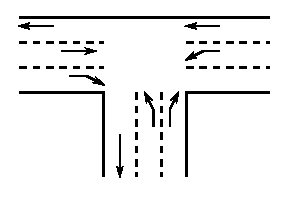
\includegraphics{pics/int3leg}\label{fig:int3leg}}
  \caption{Examples of intersections}
\end{figure}

Based on the directions of vehicles, a street can be further seperated into several traffic lanes. For example, the 4 streets in the intersection illustrated by Figure \ref{fig:int4leg} are all split into two lanes corresponding to two opposite directions. On the other hand, in Figure \ref{fig:int3leg}, the streets all consist of three lanes (Note that in this intersection, the lanes are split based on both the current and the potential directions of vehicles). A street may correspond to more than one traffic signals, but a lane can only correspond to one. Hence, the traffic lanes are more appropriate to be considered as the units of the traffic areas instead of the streets.
%Therefore, the transportation system is considered as the network of traffic lanes in this paper.
For each lane, the appropriate state variable is obviously the number of the vehicles within it, which, in this paper, is called the queue length of the traffic lane.

Now, observe that to accomplish the functionality of transportation, a vehicle need enter the transportation network from its departure point, travel from one lane to another until leaving the system at its destination. This is the fundamental of the transportation system. Hence, the dynamic of the system is reflected by the movements of vehicles. By applying the traffic flow theory \citep{nathan_h_gartner_revised_2005}, these movements can be considered as traffic flows.

Consider a transportation network including $n$ traffic lanes, $n>0$. Figure \ref{fig:flows} illustrates all traffic flows related with the lane $i$, $i\in\{1,\cdots,n\}$. $x_i$ is the queue length of lane $i$; the flow $r_i$ denotes the vehicles entering the lane $i$ from the outside; the flow $\sigma_{i,j}$ (resp, $\sigma_{j,i}$), $j\neq i$, $j\in\{1,\cdots,n\}$, represents the vehicles travel from the lane $j$ (resp, $i$) queue to the lane $i$ (resp, $j$); the flow $d_{i}$ is the output flow denoting the vehicles which leave the transportation system from the lane $i$.

\begin{figure}[ht]
  \centering
  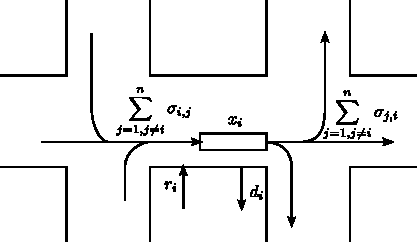
\includegraphics{pics/flows}
  \caption{The traffic flows related with the lane $i$}
  \label{fig:flows}
\end{figure}

To describe the dynamic of the transportation system from discrete-time approach, the change of the queue length $x_i$ during the interval $k$, $k\in\mathbb{N}$, is given by
\begin{equation}\label{equ:mdl_gnl_lane}
\Delta x_i(k) = l_i(k)+r_i(k)-d_i(k)
\end{equation}
where $l_i$ is the sum of all exchange flows related with lane $i$, which means
\begin{equation}\label{equ:exchange_vehicle}
 l_i(k)=\sum_{j=1,j\neq i}^{n}(\sigma_{i,j}(k)-\sigma_{j,i}(k))
\end{equation}
Equivalently, in vector form, the transportation system can be represented by the following state-space difference equation
\begin{equation}\label{equ:mdl_gnl}
\vec{x}(k+1)=\vec{x}(k)+\vec{l}(k)+\vec{r}(k)-\vec{d}(k),\quad \forall k\in\mathbb{N}
\end{equation}
where $\vec{x}=[x_1,\cdots,x_n]^T$, $\vec{l}=[l_1,\cdots,l_n]^T$, $\vec{r}=[r_1,\cdots,r_n]^T$, $\vec{d}=[d_1,\cdots,d_n]^T$, and $x_i(k)$ is the queue length of lane $i$ at the beginning of the interval $k$.

It is important to note that without any specific assumption, \eqref{equ:mdl_gnl} is a general model, which suits any kind of transportation system in any circumstance. Based on this general model, the sequel will explore the nature of transportation system from thermodynamic point of view.

\subsection{Introduction to Thermodynamic System}

The fundamental concept for analyzing the large-scale thermodynamic systems is the concept of energy. Indeed, assume that a matter with an unique temperature is called a subsystem, the thermodynamic system consists of a bunch of subsystems, which can store certain quantities of energy and are connected so that the energy can be transferred among them. Let the energy stored inside the subsystems be their state variables, these states change when the energy flows occur between the subsystems and their surroundings (including other subsystems and the outside of the system). In this paper, the work done by either the system or the environment is not concerned, hence the energy flows have only the form of heat which is driven by the temperature differences.

Based on these understandings, \citet{haddad_thermodynamic_2005} presented a discrete-time model for the large scale open thermodynamic system. Now, consider the thermodynamic system including $n$ subsystems. As shown in Figure \ref{fig:Ther_Sys}, the $i$th subsystem is denoted by $\Psi_i$, $i\in \{1,\cdots,n\}$, and its stored energy is denoted by $E_i$. Let $E_i^*>0$ be the thermal capacity of $\Psi_i$, then the temperature of $\Psi_i$ is given by
\begin{equation}\label{equ:temperature}
    T_i= {E_i}/{E^*_i}
\end{equation}

\begin{figure}[ht]
  % Requires \usepackage{graphicx}
  \centering
  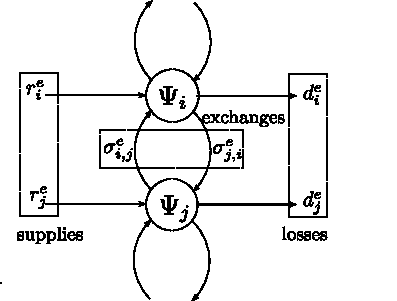
\includegraphics{pics/HModel}
  \caption{Thermodynamic system}
  \label{fig:Ther_Sys}
\end{figure}

In Figure \ref{fig:Ther_Sys}, the energy flow supplied by the outside to $i$th subsystem is denoted by $r^e_i$. The flow $\sigma^e_{i,j}$ (resp, $\sigma^e_{j,i}$), $i\neq j$, $i,j\in \{1,\cdots,n\}$, represents the transmission of energy from the $j$th (resp, $i$th) subsystem to the $i$th (resp, $j$th) subsystem. The flow $d^e_i$, $i\in \{1,\cdots,n\}$, represents the energy loss from the $i$th subsystem to the outside of the system. By combining the input, exchange and output energy flows, the dynamic of the energy $E_i$ stored by $\Psi_i$ can be given by
\begin{equation}\label{equ:Ther_Model_SubSystem}
\Delta E_i(k) = \sum_{j=1,j\neq
i}^{n}(\sigma^e_{i,j}(k)-\sigma^e_{j,i}(k))+r^e_i(k)-d^e_i(k)
\end{equation}
which equivalently infers the state-space model of the thermodynamic system
\begin{equation}\label{equ:Ther_Model}
    \vec{E}(k+1)=\vec{E}(k)+\vec{l}^e(k)+\vec{r}^e(k)-\vec{d}^e(k)
\end{equation}
where $\vec{E}(k)=[E_1(k),\cdots,E_n(k)]^T$ is the vector of the energy stored by all subsystems at the beginning of $k$th interval, $\vec{r}^e=[r^e_1,\cdots,r^e_n]^T$, $\vec{d}^e=[d^e_{1},\cdots,d^e_{n}]^T$, and $\vec{l}^e=[l^e_1,\cdots,l^e_n]^T$ represents all exchange flows such that
\begin{equation*}
l^e_i = \sum_{j=1,j\neq i}^{n}
        (\sigma^e_{i,j}-\sigma^e_{j,i}),
\; i\in \{1,\cdots,n\}
\end{equation*}

\subsection{Correspondences of Basic Concepts}

Now, by comparing the transportation model \eqref{equ:mdl_gnl} and the thermodynamic model \eqref{equ:Ther_Model}, it is clear that these two systems have many common aspects. In particular, the vehicles perform very similarly as the energy does in the thermodynamic system. Hence, the vehicles can be considered as the transportation ``energy''. Based on this fundamental correspondence, the thermodynamic concepts can be introduced into the transportation context.

Indeed, each traffic lane can contain certain amount of vehicles. The vehicles move between the connected lanes or between a lane and the outside. Obviously, the lanes are like the subsystems in the thermodynamic context, which store energy and exchange energy with their surroundings. Hence, the traffic lane is the corresponding notion of the thermodynamic subsystem and the queue lengths $x_i$ correspond to the energy stored in subsystems $E_i$, $i\in\{1,\cdots,n\}$.

The temperature is also an important thermodynamic concept. For finding its correspondence in transportation context, the corresponding notion of the thermal capacity should be firstly found. Since the lengths of traffic lanes are fixed, hence there exists a maximal capacity for each lane to contain vehicles. Let $x_i^*$, $i\in\{1,\cdots,n\}$, be the capacity of the lane $i$. It is not difficult to observe that the appropriate corresponding notion of the thermal capacity $E_i^*$ is the lane capacity $x_i^*$. Furthermore, we can define the occupancy of a lane as the proportion of the queue length to the capacity, which is given by
\begin{equation}\label{equ:occupancy}
f_i = \frac{x_i}{x_i^*},\quad i\in\{1,\cdots,n\}
\end{equation}
Compared with the equation \eqref{equ:temperature}, the occupancies $f_i$ obviously correspond to the temperatures $T_i$, $i\in\{1,\cdots,n\}$.

In summary, Table \ref{tab:notions} lists the correspondences of the basic concepts between thermodynamic and transportation systems. This analogy will provide us the opportunity to introduce thermodynamic principles into transportation context as well.

\begin{table}[ht]
\centering \caption{Correspondence of basic concepts}
\label{tab:notions}
\begin{tabular}{cc}
  \hline
  % after \\: \hline or \cline{col1-col2} \cline{col3-col4} ...
  Thermodynamic Concepts & Transportation Concepts \\
  \hline
  energy & vehicle \\
  subsystem & traffic lane \\
  energy stored in subsystems & queue lengths \\
  thermal capacity & lane capacity \\
  temperature & occupancy \\
  \hline
\end{tabular}
\end{table}

\subsection{Conservation of Vehicle (First Principle)}

The first law of thermodynamics, called the conservation of energy \citep{cengel_thermodynamics:_2001}, indicates that the energy can not be created or destroyed, it can only change forms or be transferred. Specially, the change of the energy stored in any thermodynamic system equals exactly the amount of the net energy exchange with its surroundings.

This principle also holds for the transportation system, because the change of  vehicles within a  system equals exactly the amount of the net traffic flows between the system and the outside. To show this principle more clearly, the following theorem is presented and proved based on the general transportation model \eqref{equ:mdl_gnl}.

\begin{thm}\label{thm:conservation}
Let $\vec{\epsilon} \triangleq [1,\cdots,1]^T$ be the vector whose all components are equal to $1$, and 
 define
\begin{equation}\label{equ:total_vehicle}
U \triangleq \vec{\epsilon}^T\vec{x}
\end{equation}
as the total number of the vehicles within the transportation network. Let
\begin{equation}\label{equ:all_io}
Q \triangleq \vec{\epsilon}^T(\vec{r}-\vec{d})
\end{equation}
be the number of the net vehicles moving from the outside into the transportation network. Then, the following statement holds $\forall k\in\mathbb{N}$
\begin{equation}\label{equ:conservation}
\Delta U(k) = Q(k)
\end{equation}
where $\Delta U(k)=U(k+1)-U(k)$.
\end{thm}
\begin{proof}
From \eqref{equ:mdl_gnl}, we have
\begin{align*}
U(k+1) &= \vec{\epsilon}^T\vec{x}(k+1)\\
       &=
\vec{\epsilon}^T\vec{x}(k)+\vec{\epsilon}^T\vec{l}(k)+\vec{\epsilon}
^T(\vec{r}(k)-\vec{d}(k))\\
       &= U(k)+\vec{\epsilon}^T\vec{l}(k)+Q(k)
\end{align*}
It follows
$$\Delta U(k)-Q(k) = \vec{\epsilon}^T\vec{l}$$
Now, observe that $\vec{\epsilon}^T\vec{l}(k) =\displaystyle \sum_{j=1}^{n} l_i(k)$ and since $l_i(k)=\displaystyle\sum_{j=1,j\neq i}^{n}(\sigma_{i,j}(k)-\sigma_{j,i}(k))$ in view of \eqref{equ:exchange_vehicle}, it follows
% Hence, \eqref{equ:conservation} is equivalent to
% $$\vec{\epsilon}^T\vec{l}(k)=0,\quad \forall k\in\mathbb{N}$$
% Now, because
% $$l_i(k)=\sum_{j=1,j\neq i}^{n}(\sigma_{i,j}(k)-\sigma_{j,i}(k))$$
% it infers that
\begin{align*}
\vec{\epsilon}^T\vec{l}(k)
    &= \sum_{i=1}^n (\sum_{j=1,j\neq i}^{n} \sigma_{i,j}(k)
       -\sum_{j=1,j\neq i}^{n} \sigma_{j,i}(k))\\
    &= \sum_{i=1}^n \sum_{j=1,j\neq i}^{n} \sigma_{i,j}(k)
       -\sum_{i=1}^n \sum_{j=1,j\neq i}^{n} \sigma_{j,i}(k)\\
    &= \sum_{i=1}^n \sum_{j=1,j\neq i}^{n} \sigma_{i,j}(k)
       -\sum_{j=1}^n \sum_{i=1,i\neq j}^{n} \sigma_{j,i}(k)\\
    &= 0
\end{align*}
which is the desired result.
\end{proof}

This theorem indicates that the total vehicles in the transportation system depends only on the traffic flows between the system and the outside, the exchange flows between different lanes can not change the total number of the vehicles within the network. Furthermore,\eqref{equ:conservation} implies
\begin{equation}\label{equ:conservation_ex}
U(k_2) = U(k_1)+\sum_{k=k_1}^{k_2-1}Q(k)
\end{equation}
for any $k_1,k_2\in\mathbb{N}$, $k_2>k_1$. Hence, according to \citep{willems_dissipative_1972-1}, the conservation of vehicles also implies that the transportation system \eqref{equ:mdl_gnl} is lossless with respect to the storage function \eqref{equ:total_vehicle} and the supply function \eqref{equ:all_io}.

\section{Transportation Entropy and Dissipativity}

\subsection{Second Law of Thermodynamics}

In the thermodynamic system, the directions and the quantities of the energy movements must follow some specific rules. For example, without heating equipment, a hot beverage will definitely become cooler in a cold room. Consequently, the energy can not move from cold air to the hot beverage but in the opposite direction. These phenomenons are consistent with the second law of thermodynamics (Clausius statement, \citet{clausius_mechanical_1867}):
\begin{quotation}
\it Heat can never pass from a colder to a warmer body without some other change, connected therewith, occurring at the same time.
\end{quotation}

This principle is usually connected with a special concept of \textbf{entropy}. The second law of thermodynamics can be also described by the way how the entropy of thermodynamic system changes.
% For example, the heat can be transferred from hotter objects to colder ones, but it can never go in the opposite direction. Certain phenomenons have been studied and generated the second law of thermodynamics \citep{cengel_thermodynamics:_2001}, which introduced a special concept.
In particular, Clausius proposed that the increase of the system entropy due to the input energy $Q$ from the environment is $Q/T^a$, where $T^a$ is the absolute temperature at the sport where the energy transmission happens \citep{clausius_mechanical_1867}. However, for any thermodynamic system, the actual increase of entropy is bigger than or equals to the one supplied by the environment. In other words, any thermodynamic system is creating entropy itself. This phenomenon can be presented by the following inequality
\begin{equation}\label{equ:clausius_ther_gnl}
\Delta \psi \ge \int\frac{dQ}{T^a}
\end{equation}
or its discrete-time version \citep{haddad_thermodynamic_2005}
\begin{equation}\label{equ:clausius_ther}
\psi(k+1) \ge \psi(k)+\sum_{i=1}^{n}\frac{Q_i(k)}{T^a_i(k+1)},
\forall k\in\mathbb{N}
\end{equation}
where $\psi$ is the entropy of the thermodynamic system, $Q_i(k)$ is the net energy that the $i$th subsystem absorbs from the outside during the interval $k$, and $T^a_i(k+1)$ is the absolute temperature of the $i$th subsystem at the end of interval $k$, $i\in\{1,\cdots,n\}$. \eqref{equ:clausius_ther_gnl} and \eqref{equ:clausius_ther} are also known as Clausius inequality.

 Furthermore, since the entropy is opposite to the capacity of the thermodynamic system to do useful work, it is also regarded as the measure of the system disorder \citep{balmakov_entropy_2001}. More precisely, bigger entropy indicates that the system is worse organized. Hence, the Clausius inequality also implies that the thermodynamic system always tends to become worse organized.

For the discrete-time thermodynamic model \eqref{equ:Ther_Model}, based on the Clausius inequality \eqref{equ:clausius_ther}, \citet{haddad_thermodynamic_2005} presented the formula of its entropy as follows
\begin{equation}
\psi(\vec{E}) \triangleq{\vec{E}^*}^T \ln
(a\vec{\epsilon}+\mat{P}_e\vec{E}) -\vec{\epsilon}^T\vec{E}^*\ln a
\label{equ:Ther_entropy}
\end{equation}
where $\psi(\vec{E})$ is the entropy, $\vec{E}^*=[E^*_1,\cdots,E^*_n]^T$, $a$ is a positive scalar which represents the difference between the absolute temperature and the temperature defined in \eqref{equ:temperature} so that $T^a_i=a+T_i$, $i\in\{1,\cdots,n\}$, and $\mat{P}_e$ is a diagonal matrix with diagonal elements $1/E^*_i$.

Note that this formula is identical with the Boltzmann entropy expression for statistical thermodynamics. Indeed, for any subsystem without phase transition, the entropies in different absolute temperatures ($T1$, $T2$) satisfy the following relationship \citep{cengel_thermodynamics:_2001}
\begin{equation}\label{equ:entropy_temperature}
\psi_i(T1)-\psi_i(T2)=E_i^* \ln \frac{T1}{T2},\quad \forall
i\in\{1,\cdots,n\}
\end{equation}
It is known that the absolute temperature of the $i$th subsystem equals $a+\frac{E_i}{E_i^*}$. Specially, when the subsystem stores no energy ($E_i=0$), its absolute temperature becomes $a$. Hence, \eqref{equ:entropy_temperature} implies
\begin{align}
\psi_i(E_i)&=\psi_i(0)+E_i^* \ln \frac{a+\frac{E_i}{E_i^*}}{a}
\nonumber\\
&=\psi_i(0)+E_i^* \ln (a+\frac{E_i}{E_i^*})-E_i^* \ln{a}
\label{equ:tmp_psi_1}
\end{align}
Now, according to the third law of thermodynamics, the entropy approaches zero when the stored energy approaches zero, which means
\begin{equation}\label{equ:entropy_zero}
\psi_i(0)=\lim_{E_i\rightarrow 0}\psi_i(E_i)=0
\end{equation}
Therefore, we have
\begin{equation}
\psi_i(E_i)=E_i^* \ln (a+\frac{E_i}{E_i^*})-E_i^* \ln{a}
\end{equation}
By summarizing all subsystems, the entropy of the whole system is given by
\begin{equation}
\psi(\vec{E})=\sum_{i=0}^n E_i^*\ln(a+\frac{E_i}{E_i^*})-E_i^*\ln a
\end{equation}
which infers the Haddad's formula of entropy \eqref{equ:Ther_entropy}.

Furthermore, since the entropy \eqref{equ:Ther_entropy} is not easy to apply in control issues, \citet{haddad_thermodynamic_2005} also introduced a dual notion to entropy, called ectropy, to measure the system order. The dual inequality to \eqref{equ:clausius_ther} is given by
\begin{equation}\label{equ:anti_clausius}
\phi(k+1)-\phi(k)\le \sum_{i=0}^n Q_i(k)T_i(k+1),
\forall k\in\mathbb{N}
\end{equation}
where $\phi$ is the ectropy of the thermodynamic system, $Q_i(k)T_i(k+1)$ is the input ectropy of $i$th subsystem supplied by the environment with the net input energy $Q_i(k)$, and $T_i(k+1)$ is the temperature of $i$th subsystem at the end of interval $k$. This inequality is also called anti-Clausius inequality, which, like Clausius inequality, is consistent with the second law of thermodynamics.

Anti-Clausius inequality indicates that in any circumstance, any thermodynamic system is destroying its ectropy so that the increase of the ectropy is always less than the one supplied from its surroundings. Opposite with the entropy, the ectropy measures the capacity of the system to do useful work, and bigger ectropy corresponds to better organization of the system.

For the discrete-time thermodynamic model \eqref{equ:Ther_Model}, based on the anti-Clausius inequality \eqref{equ:anti_clausius}, \citet{haddad_thermodynamic_2005} presented the formula of the ectropy as follows
\begin{align}
\phi(\vec{E})&\triangleq\frac{1}{2}\vec{E}^T \mat{P}_e \vec{E}
\label{equ:Ther_ectropy}
\end{align}

Contrary to the energy, the entropy and the ectropy are both non-conservative notions. Specially in the isolated system, the sum of energy always keeps constant, but the entropy tends to increase while the ectropy tends to decrease. Besides, it is important to note that the ectropy \eqref{equ:Ther_ectropy} has the form of Lyapunov function, which is more useful in control issues than the entropy.

\subsection{Transportation Entropy}
% The above section has analogized the transportation system to the thermodynamic system, which encourages us to introduce entropy concept into transportation context to be the evaluation of the system performance.
The correspondence between transportation systems and thermodynamic systems encourages us to introduce the entropy concept into transportation context in order to evaluate the system performances. However, the problem is that there is no natural principle in transportation context that corresponds to the second law of thermodynamics. As a matter of fact, the directions of vehicles are determined by the drivers, there is no such rule that the vehicles only move from more crowded lanes to less crowded ones. Hence, we can not introduce transportation entropy based on certain principles as it is defined in the thermodynamic context. However, Nevertheless, based on the correspondences of certain concepts, such as energy and temperature, we can still simply introduce the formulas in the thermodynamic system to present the transportation entropy as the measure of the system disorder.

To do this, the significations of orders in these two systems must be firstly compared. Indeed, in thermodynamic context, higher order means higher capacity to do useful work, which is related with bigger temperature differences between subsystems. For example, in a thermodynamic system including two subsystems, if more energy concentrates on one single subsystem to generate bigger temperature difference, the quantity of the potential energy movements is bigger, which means that the system can generate more useful work. In this case, the system is regarded as better organized and has higher order. But on the converse, the bigger differences between the occupancies correspond to lower order in transportation context. Indeed, for a general transportation network, if more vehicles concentrate in only a few lanes, it has bigger probability to generate congestions in these lanes and the other lanes are wasted. In this case, the system is regarded as worse organized and has lower order.

Moreover, the energy input to the thermodynamic system brings more capacity to do useful work, which increases the order. However, in transportation context, the vehicle input brings more potential opportunity to generate congestions, which decrease the order. For an isolated thermodynamic system without energy input, the disorder (entropy) can only increase until it reaches equilibrium. On the converse, if, at a certain moment, the transportation system has no vehicle input, the system will keep dissipating the present vehicles and consequently become better organized.

In conclusion, the order significations of these two systems are opposite, which means the disorder in the transportation system corresponds to the order in the thermodynamic system. In other words, the transportation entropy (resp, ectropy) should correspond to the thermodynamic ectropy (resp, entropy). Therefore, according to the thermodynamic ectropy and entropy formulas \eqref{equ:Ther_ectropy}, \eqref{equ:Ther_entropy}, the \textbf{transportation entropy and ectropy} are defined respectively as
\begin{align}
\label{equ:Tran_entropy}
\psi(\vec{x}) &\triangleq \frac{1}{2}\vec{x}^T \mat{P} \vec{x}\\
\phi(\vec{x}) &\triangleq{\vec{x}^*}^T \ln
(a\vec{\epsilon}+\mat{P}\vec{x}) -\vec{\epsilon}^T\vec{x}^*\ln a
\label{equ:Tran_ectropy}
\end{align}
where $\psi(\vec{x})$ is transportation entropy, $\phi(\vec{x})$ is transportation ectropy, $a$ is a positive scalar, $\mat{P}$ is the diagonal matrix with the diagonal elements $1/x_i^*$, and $\vec{x}^*=[x_1^*,\cdots,x_n^*]^T$. Here, the logarithm of a vector is the vector of the logarithm of each component.
% Since the Haddad's formula of entropy is identical with the Boltzmann's one, the definitions of the transportation entropy and ectropy can also be considered as consistent with Boltzmann's approach.

% It is important to note that the entropy \eqref{equ:Tran_entropy} is a Lyapunov candidate function, which is much more useful in control issues than the ectropy \eqref{equ:Tran_ectropy}. Hence, it will be the major emphasis of the sequel.

The formula of the transportation entropy \eqref{equ:Tran_entropy} comes only from the thermodynamic system, but we have not shown its signification in the transportation context. To do this, consider the transportation network as a service provider and consider the vehicles traveling within it as its customers. Hence, the order of transportation network should be the sum of the qualities of the services provided to all vehicles, and the disorder is, of course, the opposite. Clearly, the services that the vehicles obtain from the urban transportation system are the traffic routes, and the qualities are evaluated by how fast the vehicles can pass these routes. Figure \ref{fig:d_q} shows the flow-density diagram based on kinetic wave model, where $\rho_m$ is the jam density, $\nu$ is the speed and $\nu_m$ is the free-flow speed \citep{ukkusuri_robust_2010}. It is observed that the traffic flow and the speed can be considered as functions of the traffic density. Precisely, the bigger traffic density generates 
the smaller speed and hence prolongs the delay. Indeed, despite the habits of drivers, any vehicle need spend more time to pass more crowded lanes. This indicates that the traffic densities are opposite to the qualities of services provided by the transportation network, hence they correspond to the system disorder.

\begin{figure}[ht]
  \centering
  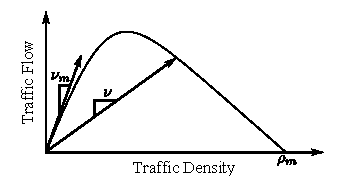
\includegraphics[height=3cm]{pics/d-q}\\
  \caption{Density-flow chart}
  \label{fig:d_q}
\end{figure}

Now, let $I(k)$ be the sum of the traffic densities that all vehicles meet at the instant $k$ in the network. For vehicles in the lane $i$, let $\rho_i(k)$ denote their traffic density at time $k$, $i\in \{1,\cdots,n\}$. Hence, we have
$$I(k)=\sum_{i=1}^{n} x_i(k)\rho_i(k)$$
Furthermore, since $\rho_i(k)=x_i(k)/h_i$ where $h_i$ is the length of the lane $i$, $i\in \{1,\cdots,n\}$, the sum of the traffic densities of all vehicles is finally restated as
\begin{equation}
\label{equ:quality_service}
I(k)=\sum_{i=1}^{n}
\frac{x_i(k)^2}{h_i}=\vec{x}(k)^T\mat{P}_h\vec{x}(k)
\end{equation}
where $\mat{P}_h$ is the diagonal matrix with the diagonal elements $1/h_i$. Since $x_i^*=\frac{h_i}{h_{veh}}$, where $h_{veh}$ is the average car length, it follows
\begin{equation}
I(k) = \sum_{i=1}^{n}\frac{x_i(k)^2}{h_{veh} x_i^*}
= \frac{2}{h_{veh}} \frac{1}{2}\vec{x}(k)^T\mat{P}\vec{x}(k)
= \frac{2}{h_{veh}} \psi(k)
\end{equation}

This indicates that the transportation entropy is proportional to the traffic densities $I(k)$ and hence it becomes now clear that this  transportation entropy  is an appropriate measurement of system disorder.
% It is also important to note that the entropy \eqref{equ:Tran_entropy} is a Lyapunov candidate function, which is very useful in control issues.

% \subsection{Dissipativity of Entropy}

% Though the second law of thermodynamics can not be applied in transportation context naturally, we still wonder whether it can be achieved in certain conditions. The major motive is that the transportation disorder corresponds to the thermodynamic order. If the transportation system has similar principle with the second law of thermodynamics, it will have the tendency to decrease its disorder and become better organized. More precisely, if the direction of the net traffic flow between any two transportation areas is from the more crowded one to the less crowded one as the energy does in the thermodynamic system, all congestions within the transportation network will tend to be evacuated.
% 
% Now, consider the anti-Clausius inequality \eqref{equ:anti_clausius} and its meaning in thermodynamic context, it can be stated that the idea is to achieve the phenomenon that the increase of the transportation entropy is always beneath its supply from the outside. In other words, the corresponding version of anti-Clausius inequality should be presented and verified.

Now, in transportation context, the input vehicles bring disorder to the system. This supplied disorder depends on not only the number of the input vehicles, but also the distribution of them. The vehicles which enter the more crowded lanes bring more disorder than the ones with same quantity which enter the less crowded lanes. Since the occupancies represent how the lanes are crowed, it is natural to measure the supplied entropy with respect to the input flows and the occupancy factors. Let $\vec{f}=[f_1,\cdots,f_n]^T$ be the vector of all occupancies. Note that because $\vec{f}(k)$ corresponds to the beginning of the interval $k$ while $\vec{f}(k+1)$ corresponds to the end of it, the supplied entropy in the interval $k$ should correspond to $\vec{f}(k+1)$ rather than $\vec{f}(k)$. So, we define
$$S(k)=\vec{f}(k+1)^T\vec{r}(k)$$
as the supplied entropy in the interval $k$. Furthermore, since $\vec{f}=\mat{P}_x\vec{x}$ in view of \eqref{equ:occupancy}, the supplied entropy is restated as
\begin{equation}\label{equ:supply}
    S(k)=\vec{x}(k+1)^T \mat{P} \vec{r}(k)
\end{equation}
Now, similar with the anti-Clausius inequality \eqref{equ:anti_clausius}, we propose its corresponding version in transportation context as follows
\begin{equation}\label{equ:dissipative}
\psi(\vec{x}(k+1))-\psi(\vec{x}(k)) \leq S(k),\quad \forall
k\in\mathbb{N}
\end{equation}
If this inequality is verified, the transportation system has the tendency to decrease its disorder and become better organized.

Furthermore, according to the \citet{willems_dissipative_1972} and \citet{hill_dissipative_1980}, \eqref{equ:dissipative} also implies the dissipativity with the entropy \eqref{equ:Tran_entropy} as the storage function and with \eqref{equ:supply} as the supply function. In this case, \eqref{equ:dissipative} is called dissipation inequality. Figure \ref{fig:trans_dis} illustrates this dissipativity of system disorder. Indeed, the input flows bring disorder to the transportation system to make it worse organized. At the same time, the appropriate traffic signal control dissipates the traffic so that the system stores only a part of this input disorder.
\begin{figure}[ht]
  \centering
  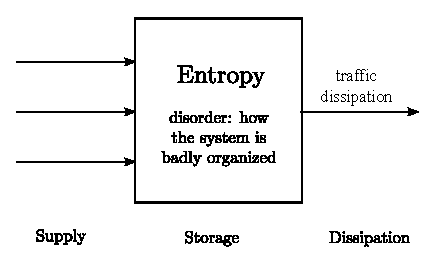
\includegraphics{pics/trans_dis}\\
  \caption{Dissipativity of transportation entropy}
  \label{fig:trans_dis}
\end{figure}

This dissipativity implies that the storage of the system disorder is always smaller than or equal to the supplied one from the outside. In other words, if this dissipative phenomenon exists in the transportation system, the system disorder will tend to decrease and hence the system will tend to become better organized.

This dissipativity does not exist naturally. But, it is known that the traffic signals have the ability to control the traffic flows. Therefore, it is possible that under certain control schemes, the traffic signals can verify the dissipation inequality \eqref{equ:dissipative}. This inequality can be considered as one of objectives for traffic signal control.

\section{Nominal Situation and Equilibrium}

In the researches about thermodynamic systems, the closed system, which has no exchange with the environment, is one of the most studied subjects. Indeed, the closed thermodynamic system has special features. For example, in any closed thermodynamic system, the ectropy (resp, entropy) keeps decreasing (resp, increasing) until reaching the equilibrium state when all connected subsystems have the same temperature. The equilibrium also corresponds to the minimal possible ectropy and maximal possible entropy. Since the ectropy is a Lyapunov function, the closed thermodynamic system is Lyapunov stable \citep{haddad_thermodynamic_2005}.

Unfortunately, the transportation system is always open. In fact, the openness is required by the functionality of the transportation. There is no such thing as closed transportation system. However, there exists nominal situation \citep{diakaki_multivariable_2002} in the transportation network which has some common features with the closed thermodynamic system. The nominal situation means that with certain traffic demands and certain traffic signal settings, the input vehicles equals the output vehicles for each traffic lane, in other words, the queue lengths of all traffic lanes keep constant. In this paper, these certain traffic demands are called nominal inputs from the outside, denoted by
$$\vec{r}^N=\{r_1^N,\cdots,r_n^N\}$$
Obviously, in the nominal situation, the net exchange between the transportation system and the outside equals zero in each cycle, that means
\begin{equation}\label{equ:nominal_exchange}
Q(k)\equiv 0, \quad \forall k\in\mathbb{N}
\end{equation}
Since the transportation system is lossless with the storage function $U$ and the supply function $Q$, \eqref{equ:nominal_exchange} infers that the total amount of vehicles $U$ within the whole system keeps constant in the nominal situation. This is very similar with the closed thermodynamic system which has zero exchange of energy with the environment.
% Hence, we propose that the nominal situation of the transportation system can be analogized to the closed status of the thermodynamic system.

Note that \citet{de_oliveira_multi-agent_2010} have presented some effective procedures to estimate the nominal parameters for the general transportation system, hence it is reasonable to assume the availability of the nominal situation in general.

Now, define the disturbances of the transportation system as the difference between the real input flows and the nominal ones, which is given by
\begin{equation}
\vec{\omega}(k)\triangleq\vec{r}(k)-\vec{r}^N, \quad \forall
k\in\mathbb{N}
\end{equation}
Since the nominal situation of transportation system is similar to the closed status of thermodynamic system, the disturbances $\vec{\omega}$ are more appropriate than the input traffic flows $\vec{r}$ to correspond to the input energy in the thermodynamic system, specially when we consider the dissipativity phenomenon.

Hence, let
\begin{equation}\label{equ:supply_omega}
  S_\omega(k) = \vec{x}(k+1)^T \mat{P} \vec{\omega}(k)
\end{equation}
be the new supply function with respect to $\vec{\omega}$. Consequently, the dissipativity presented in previous section can be modified to the one with the entropy \eqref{equ:Tran_entropy} as the storage function and with \eqref{equ:supply_omega} as the supply function. Note that this new dissipativity is the sufficient condition of the previous one, which is stated in the following theorem.

\begin{thm}
If the transportation system described by the difference equation \eqref{equ:mdl_gnl} is dissipative with respect to the storage function \eqref{equ:Tran_entropy} and the supply function \eqref{equ:supply_omega}, then the system is also dissipative with respect to the same storage function and the supply function \eqref{equ:supply}.
\end{thm}
\begin{proof}
The dissipation inequality related with the storage function (\ref{equ:Tran_entropy}) and the supply function
(\ref{equ:supply_omega}) is
\begin{equation}\label{equ:dissipative_omega}
  \psi(\vec{x}(k+1))-\psi(\vec{x}(k)) \leq S_\omega(k)
\end{equation}
Since $\vec{\omega}(k)=\vec{r}(k)-\vec{r}^N$, it follows
\begin{align*}
S_\omega(k) &= \vec{x}(k+1)^T \mat{P} (\vec{r}(k)-\vec{r}^N)\\
    &= \vec{x}(k+1)^T \mat{P} \vec{r}(k)-\vec{x}(k+1)^T\mat{P}\vec{r}^N
\end{align*}
Since the nominal inputs and all queue lengths are non-negative, this infers
$$S_\omega(k)\leq \vec{x}(k+1)^T \mat{P} \vec{r}(k) = S(k)$$
So, the conclusion follows.
\end{proof}
% Now, the second law of thermodynamics corresponds to this new dissipativity.
This theorem also implies that the dissipativity with the supply function $S_\omega(k)$ is more strict than the one with the supply function $S(k)$. Hence, by taking the new dissipativity as the objective instead of the previous one, the traffic signal control can generate better performances.

Finally, we close this section by introducing the concept of thermal equilibrium into the transportation context. For a closed thermodynamic system, if a pair of connected subsystems have different temperatures, the energy transmission will emerge between them so that their temperatures tend to approximate. After enough time, all connected subsystems will have the same temperature so that no energy movement can emerge any more. In other words, the system loses all its capacity to do useful work in this moment. This particular state is called thermal equilibrium state \citep{cengel_thermodynamics:_2001}, which also corresponds to the maximal entropy and minimal ectropy in the closed thermodynamic system.

This concept of equilibrium can be also introduced into the transportation context to denote the state when the occupancies of all traffic lanes are the same, which implies that the vehicles are uniformly distributed within the whole transportation area in the transportation equilibrium. Mathematically, the transportation equilibrium means
\begin{equation}\label{equ:equilibrium}
\frac{x_1}{x_1^*}=\cdots=\frac{x_n}{x_n^*}=\alpha
\end{equation}
where
$$\alpha = \frac{\vec{\epsilon}^T\vec{x}}{\vec{\epsilon}^T\vec{x}^*}
\in[0,1]$$
% It can be easily proved that the transportation equilibrium
% corresponds to the minimization of the transportation entropy with
% certain amount of traffic.
The relationship between the transportation equilibrium and the transportation entropy is stated in the following theorem.

\begin{thm}\label{thm:entropy_equilibrium}
Assume that the total amount of vehicles $N$ is given, the transportation entropy \eqref{equ:Tran_entropy} is minimized when the system reaches the equilibrium state \eqref{equ:equilibrium}.
\end{thm}
\begin{proof}
To minimize the entropy, consider the problem
\begin{align}\label{equ:pro_min_psi}
\min\; &\psi(\vec{x}) = \frac{1}{2}\vec{x}^T\mat{P}\vec{x}\\
s.t.\; &\sum_{i=1}^n x_i = N \nonumber
\end{align}
Since $\psi(\vec{x})$ is a convex function, by applying the method of Lagrange multipliers to solve the problem \eqref{equ:pro_min_psi}, we have the equivalent unconstrained problem:
$$\min J(\vec{x},\beta) =
\frac{1}{2}\vec{x}^T\mat{P}\vec{x}+\beta(\sum_{i=1}^n x_i - N)$$
whose solution can be obtained by solving the equations
\begin{align}
\label{equ:tmp_min_J_1}
\frac{\partial J}{\partial x_i} &= \frac{x_i}{x_i^*}+\beta =0,
i\in\{1,\cdots,n\}\\
\label{equ:tmp_min_J_2}
\frac{\partial J}{\partial \beta} &= \sum_{i=1}^n x_i - N =0
\end{align}
Now, from \eqref{equ:tmp_min_J_1}, we have
$$\frac{x_1}{x_1^*}=\cdots=\frac{x_n}{x_n^*}=-\beta
$$
Apparently, $\beta$ can only equal to $-\alpha$, which completes the proof.
\end{proof}

Transportation equilibrium also implies that no particular concentration of vehicles exists in the system and hence the possibility to emerge congestion is extremely low. The transportation equilibrium is actually the ideal state for the transportation system and the ideal objective shared by all dynamic traffic signal control strategies.

\section{Approach of Shannon's Entropy}

The above studies analogized the transportation system to thermodynamic system by regarding the vehicles as the energy. Beside this approach, it is noticed that the researches of thermodynamics have been expanded to the domains other than pure physical systems. In particular, Shannon has connected the entropy with the concept of information \citep{Shannon1948}. This work encourages us to explore the nature of the transportation system from the perspective of information theory, which is the emphasis of this section.

\subsection{Information of Transportation System}

As a very important expansion of the statistical thermodynamics, Shannon's entropy measures the information gained by measuring certain random variable \citep{Shannon1948}. In particular, for a random variable $Y$ with possible states $\{y_i\}$, if the probability distribution of $Y$ over its possible states is $\{p_i\}$, then the information gained by measuring $Y$ can be given by the relative Shannon's entropy as follows
\begin{equation}\label{equ:shannon}
H(Y) = -\sum p_i \log_2 p_i
\end{equation}
Note that by using $2$ as the base of logarithm, the unit of the information \eqref{equ:shannon} is $\unit{bit}$.

In transportation context, the most important information is the occupancy status of the traffic areas, which can infer the degree of crowdedness. Since the Shannon's entropy measures the information gained by necessary measurement, it means the Shannon's entropy represents the unknown information or in other words the unpredictability of the information. In the transportation system, if the vehicles move more fast, it is more difficult to predict the occupancy of certain traffic areas. Therefore, if the transportation system functions more smooth, the information measured by the Shannon's entropy will be greater.

Now, consider a single spot of lane $i$, $\forall i\in\{1,\cdots,n\}$. Suppose that the queue length $x_i$ and the lane capacity $x_i^*$ are both known but there is no direct measurement on this specific spot. It can be inferred that the possibility that this spot is occupied is $\frac{x_i}{x_i^*}$, and the possibility of the otherwise case is $(1-\frac{x_i}{x_i^*})$. Hence, the information gained by measuring this spot is
$$-[\frac{x_i}{x_i^*} \log_2 \frac{x_i}{x_i^*}+(1-\frac{x_i}{x_i^*})
\log_2 (1-\frac{x_i}{x_i^*})]
$$
For the whole lane $i$, the information of all spots' occupancies can be given by
\begin{equation}\label{equ:info_lane_h}
H_i(x_i) = -h_i[\frac{x_i}{x_i^*} \log_2
\frac{x_i}{x_i^*}+(1-\frac{x_i}{x_i^*}) \log_2 (1-\frac{x_i}{x_i^*})]
\end{equation}
Since $h_i=h_{veh} x_i^*$ and the average car length $h_{veh}$ is considered fixed generally, \eqref{equ:info_lane_h} can be simplified to
\begin{align}
H_i(x_i) &= -x_i^*[\frac{x_i}{x_i^*} \log_2
\frac{x_i}{x_i^*}+(1-\frac{x_i}{x_i^*}) \log_2
(1-\frac{x_i}{x_i^*})] \nonumber\\
&=-[x_i \log_2 \frac{x_i}{x_i^*}+(x_i^*-x_i) \log_2
(1-\frac{x_i}{x_i^*})] \label{equ:info_lane}
\end{align}
By summarizing all lanes, we have the information of the entire system as follows
\begin{align}
H(\vec{x}) &= \sum_{i=1}^n H_i(x_i)\nonumber\\
&= - \sum_{i=1}^n [x_i \log_2 \frac{x_i}{x_i^*}+(x_i^*-x_i) \log_2
(1-\frac{x_i}{x_i^*})]\label{equ:info_network_sum}
\end{align}
which can be further restated as the vector expression
\begin{equation}\label{equ:info}
H(\vec{x}) = -\vec{x}^T\log_2\mat{P}\vec{x}
-(\vec{x}^*-\vec{x})^T\log_2(\vec{\epsilon-\mat{P}\vec{x}})
\end{equation}
We define this expression as the information of transportation system. The sequel will discuss its signification in transportation context.
% It represents the uncertainty or unpredictability of the system crowdedness by knowing only the queue lengths and the lane capacities.

\subsection{Signification}

The information \eqref{equ:info} of transportation system comes from the consideration of the occupancies of traffic areas. Precisely, it measures the uncertainty of the occupancies. If the occupancy of a traffic spot is more uncertain, which means it is more difficult to predict whether there is a vehicle in this spot without direct observation, it implies that this spot has higher fluidity. In other words, the greater information \eqref{equ:info} implies the higher fluidity of the whole transportation system. It is clear that the fluidity corresponds to the transportation functionality. Hence, the information of transportation system is related with the transportation functionality of the system. The sequel will discuss this relationship in detail.

% FOR A LANE
First, consider a single lane $i$, $i\in\{1,\cdots,n\}$, its information $H_i$ due to all possible queue length $x_i$ is illustrated in Figure \ref{fig:info_lane}. Observe that when the lane is empty ($x_i=0$), the information equals zero ($H_i=0$). This is because any spot within this lane is certainly not occupied by a vehicle. This lane is extremely clean in this case. However, since no vehicle travels inside, no transportation behavior appears in this lane. In other words, the system contributes nothing to the transportation functionality with zero usage.

\begin{figure}[ht]
  \centering
  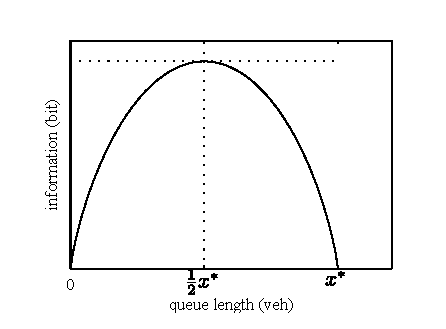
\includegraphics{pics/lane}\\
  \caption{Information vs queue length for a lane}
  \label{fig:info_lane}
\end{figure}

On the other hand, when the lane is totally occupied ($x_i=x_i^*$), since the occupancy of any spot is also certain in this case, the information $H_i$ also equals zero. The usage of the system is extremely high in this case. But, because there is no space to move, the transportation behavior can not happen either. Hence, with complete crowdedness, the system also contributes nothing to the transportation functionality.

Now, we can summarize that the transportation functions only under these two conditions:
\begin{enumerate}
  \item[\textbf{C1}] there are vehicles; \label{list:c1}
  \item[\textbf{C2}] there are free spaces to allow the vehicles to move. \label{list:c2}
\end{enumerate}
In other words, the transportation functionality depends on the balance between usage and free spaces. Therefore, only when $0<x_i<x_i^*$, these two conditions are both verified so that this lane can contribute to the transportation functionality.

Observe that only when $0<x_i<x_i^*$, the information $H_i$ becomes positive because the occupancies are uncertain in this case. Specially, $H_i$ maximizes when the lane is half-occupied ($x_i=x_i^*/2$). It can be concluded that, for a lane, its information $H_i$ reflects the balance between usage and free spaces, hence the information corresponds to the transportation functionality.

% FOR NETWORK
Beside the relationship with the number of vehicles, the information of a transportation network also relies on the distribution of vehicles over different lanes if the total amount of vehicles is given.
% Then, we consider the relationship between the transportation information and the distribution of vehicles over different lanes.
For example, consider a system including two lanes. Let $x_1$, $x_2$ be the queue lengths and let $x_1^*$, $x_2^*$ be the capacities. Suppose $x_1^*<x_2^*$ and the sum $N=x_1+x_2$ is fixed. Figure \ref{fig:info_twolane} shows the information due to $x_1$ in three cases: $N\le x^*_1\le x^*_2$, $x^*_1\le N\le x^*_2$ and $x^*_1\le x^*_2\le N$. The information maximizes in certain point $x_p$, which is given by in all three cases
$$x_p = \frac{N}{x_1^*+x_2^*} x_1^*$$
This maximal point happens to mean that the vehicles are distributed uniformly in these two lanes. Clearly, the information reflects the balance between these two lanes as well.

\begin{figure}[ht]
  \centering
  \subfigure[$N\le x^*_1\le x^*_2$]
  {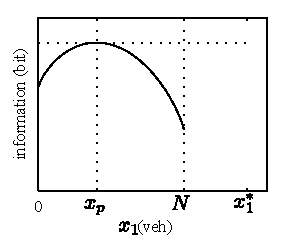
\includegraphics[width=0.3\textwidth]{pics/twolane_s}}
  \subfigure[$x^*_1\le N\le x^*_2$]
  {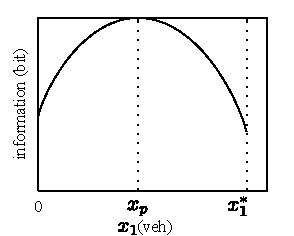
\includegraphics[width=0.3\textwidth]{pics/twolane_m}}
  \subfigure[$x^*_1\le x^*_2\le N$]
  {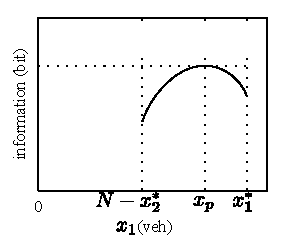
\includegraphics[width=0.3\textwidth]{pics/twolane_l}}\\
  \caption{Information of two lanes with fixed total vehicles}
  \label{fig:info_twolane}
\end{figure}

Furthermore, the following theorem indicates that for any large-scale transportation network, if the total amount of vehicles is given, the information maximizes when the vehicles are distributed uniformly.

\begin{thm}\label{thm:info_max}
For any transportation network including $n$ lanes, assume that the total amount of vehicles $N$ is given, the transportation information \eqref{equ:info} is maximized when the vehicles are distributed uniformly.
\end{thm}
\begin{proof}
To maximize the information, consider the problem
\begin{align}\label{equ:pro_max_info}
\max\; &H(\vec{x}) = -\vec{x}^T\log_2\mat{P}\vec{x}
-(\vec{x}^*-\vec{x})^T\log_2(\vec{\epsilon-\mat{P}\vec{x}})\\
s.t.\; &\sum_{i=1}^n x_i = N \nonumber
\end{align}
Since
\begin{align*}
\frac{\partial^2 H}{\partial x_i\partial x_j} &= 0,\;\forall
i,j\in\{1,\cdots,n\},i\neq j\\
\frac{\partial^2 H}{\partial x_i^2} &= -\frac{1}{\ln
2}(\frac{1}{x_i}+\frac{1}{x_i^*-x_i})<0,\;\forall i\in\{1,\cdots,n\}
\end{align*}
we know that $H(\vec{x})$ is a concave function. By applying the method of Lagrange multipliers to solve the problem \eqref{equ:pro_max_info}, we have the equivalent unconstrained problem:
$$\max J(\vec{x},\beta) =
-\vec{x}^T\log_2\mat{P}\vec{x}
-(\vec{x}^*-\vec{x})^T\log_2(\vec{\epsilon-\mat{P}\vec{x}})
+\beta(\sum_{i=1}^n x_i - N)$$
whose solution can be obtained by solving the equations
\begin{align}
\label{equ:tmp_max_J_1}
\frac{\partial J}{\partial x_i} &=
-\log_2\frac{x_i}{x_i^*}+\log_2(1-\frac{x_i}{x_i^*})+\beta =0,
\forall i\in\{1,\cdots,n\}\\
\label{equ:tmp_max_J_2}
\frac{\partial J}{\partial \beta} &= \sum_{i=1}^n x_i - N =0
\end{align}
Now, \eqref{equ:tmp_max_J_1} can easily infer that
$$\frac{x_1}{x_1^*}=\cdots=\frac{x_n}{x_n^*}=\frac{1}{1+2^{-\beta}}
$$
Apparently, this implies the uniform distribution of vehicles, which completes the proof.
\end{proof}

Since the information maximizes when the vehicles are distributed uniformly and the information is a concave function, it is implied that the information reflects the balance of vehicles between different traffic lanes. Consider that, if the vehicles are distributed more uniformly, the traffic lanes are used more equally for the transportation functionality. Hence, by considering the distribution of vehicles over the network, the information is also related to the transportation functionality.

% The uniform distribution of vehicles implies that all traffic areas are equally used for the transportation functionality, there is no waste and no overuse. This state leads to the  highest overall liquidity of the transportation system.

Now, by combining above analysis, the information of transportation system reflects the balance between usage and free spaces, and reflects the balance between different traffic lanes. These two balances together determine the contribution of the system to the transportation functionality. In other words, the information of transportation system is the appropriate measurement of the transportation functionality for the system.

\subsection{Comparison Between Entropy and Information}

% ENTROPY: CONTROL OBJECTIVE
% INFORMATION: FUNCTIONALITY OF TRANSPORTATION

From the approaches of classical thermodynamics and expanded Shannon's information theory, this paper has presented the entropy \eqref{equ:Tran_entropy} and the information \eqref{equ:info} for the transportation system. We close this section by comparing these two novel concepts.

From different bases, the significations of these two concepts are very different. By considering the vehicles as the energy, the transportation entropy is presented based on the parallelism between the transportation system and the thermodynamic system. It is the measure of system disorder, which is proportional to the sum of traffic densities of all vehicles and therefore opposite to the service quality supplied by the system to the vehicles. Obviously, the entropy focuses on the services obtained by the vehicles and it is desired to be reduced.

But on the other hand, the information of transportation system measures the system contribution to the transportation functionality. It comes from the consideration of the occupancy states of all traffic areas. Different from the entropy, the information focuses on the performance of the transportation system (not the vehicles) and it is desired to be increased.

This difference appears in their relationships with the queue lengths. The entropy \eqref{equ:Tran_entropy} is a monotonic function of queue lengths. It is obvious that every vehicle hopes to share the traffic resources with as less vehicles as possible. But, the transportation information \eqref{equ:info} approaches zero when the number of vehicles approaches zero because transportation functionality needs the vehicles and too few of them will lead to big waste of traffic infrastructures. More precisely, the considerations based on the entropy desire that the vehicles are reduced as many as possible, while the maximization of the information desires that the lanes are half-occupied.

Apparently, the transportation entropy is more appropriate to be used in traffic signal control, because the fundamental aim of the traffic signals is to enhance the service quality for the vehicles. On the other hand, the transportation information is better to evaluate the performance of the transportation system itself. The transportation system with bigger information means it contributes more to the transportation functionality for the society.
% In our opinion, the information \eqref{equ:info} is also more useful in the domains, such as the transportation infrastructure design, the urban planning, etc.

% At last, we note that these two notions have common features to consider the distribution law of vehicles. No matter to minimize the entropy or to maximize the information, the vehicles are both desired to be distributed uniformly, which implies that the uniform distribution of vehicles is beneficial to both the vehicles and the transportation system.

\section{Conclusion}

This paper has studied the transportation system from the thermodynamic and information theory perspectives. First, the comparison between the thermodynamic system and the transportation system showed that they are very similar by regarding the vehicles as the energy and regarding the traffic lanes as the thermodynamic subsystems. Hence, this paper has introduced the thermodynamic concepts into the transportation context. In particular, it has been demonstrated that the transportation system can have a similar notion of the entropy to measure the system disorder. By considering this notion as the storage function, this paper has presented a dissipativity law for the transportation system to decrease its disorder and hence render the system better organized. Though it is not verified naturally, it can be used as the objective of the traffic signal control. Furthermore, the equilibrium state was also introduced into the transportation context to represent the uniform distribution of the vehicles. Beside the classical thermodynamic approach, this paper also applied the Shannon's point of view to present the information of transportation system, which can measure the transportation functionality and hence can be a good means to evaluate the system.

In summary, this paper has constructed a novel thermodynamic and information theory point of view in traffic engineering. This work is a completely new attempt to discover the nature of the transportation system. The contributions of this paper provide a new approach to design better traffic signal control strategies.

\bibliographystyle{model5-names}
\bibliography{zhou_refs}

\end{document}
